\chapter{Общие подходы к решению задачи трансфера SAR $\rightarrow$ Optical и их развитие}
\label{sec:Chapter3} \index{Chapter3}

\section{Парные методы на основе условных GAN (семейство Pix2Pix)}
\label{sec:pix2pix_review}

Парные (контролируемые) методы перевода изображений опираются на наличие строго выровненных пар «вход – целевое изображение». В задаче трансляции SAR $\rightarrow$ оптика это означает, что для каждого радарного снимка имеется полученный в той же геометрии и приблизительно в то же время оптический снимок, выступающий эталоном.

Основу данного направления заложила архитектура Pix2Pix, предложенная Исолой и др. \cite{isola2017image}, которая впервые показала, что условная генеративно-состязательная сеть способна решать широкий круг задач перевода изображений с одним и тем же набором гиперпараметров.

\begin{figure}[!ht]
    \centering
    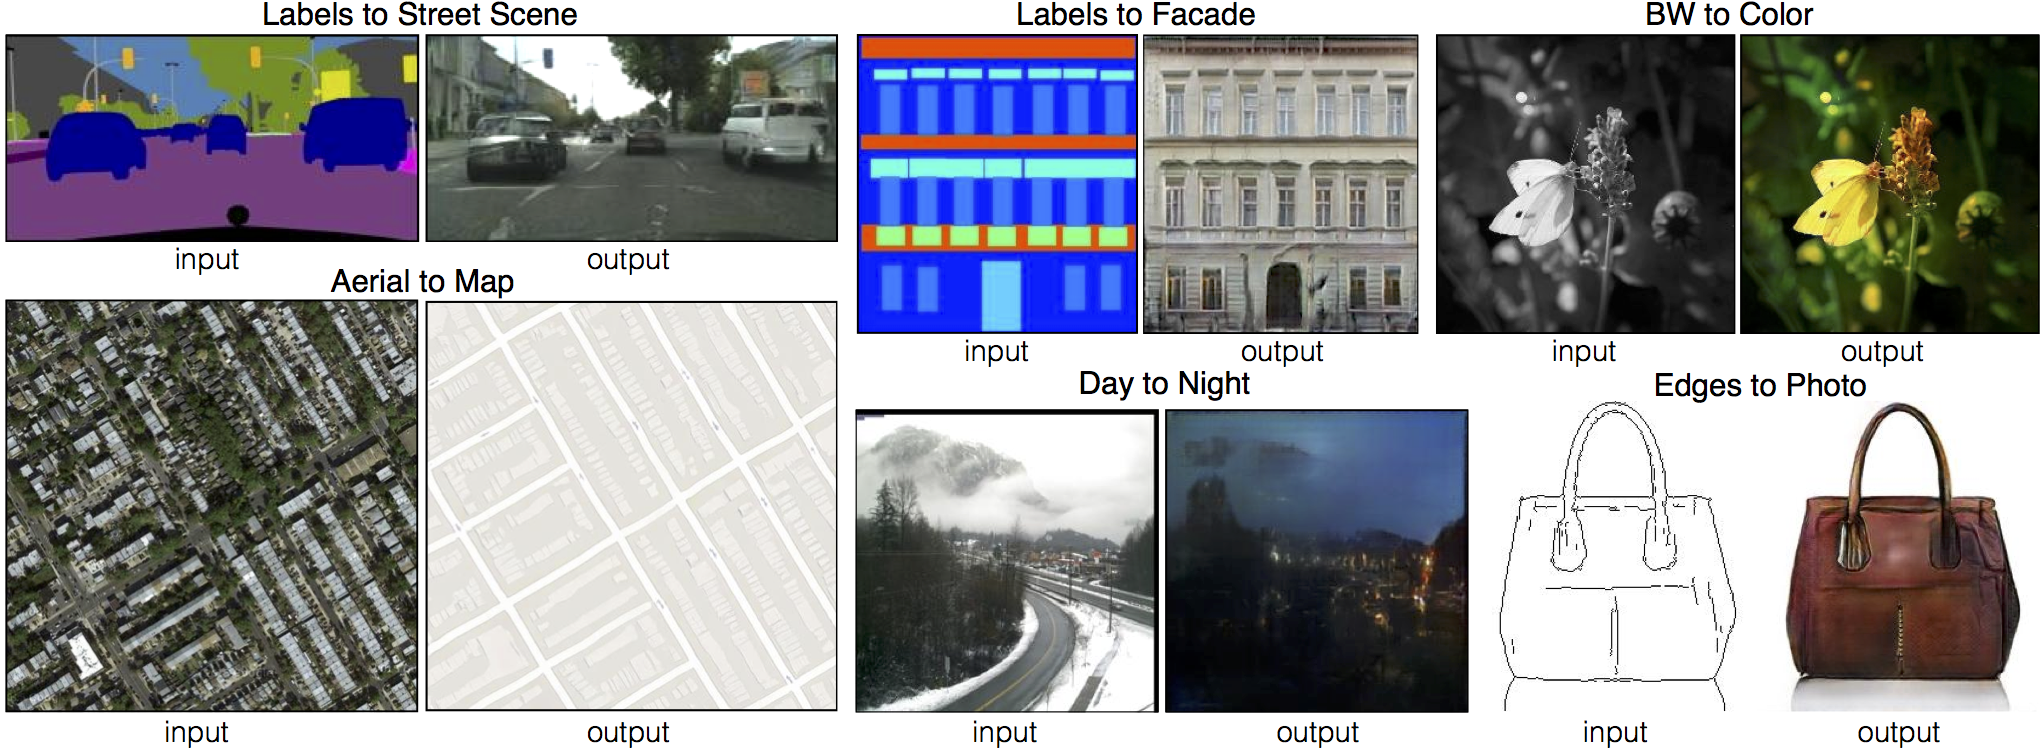
\includegraphics[width=1\linewidth]{images/pix2pix/pix2pix_example.png}
    \caption{Примеры областей использования модели Pix2Pix}
    \label{fig:pix2pix_example}
\end{figure}

\subsection{Базовая архитектура и принцип обучения}

Классическая модель Pix2Pix (рис.~\ref{fig:pix2pix_arch}) состоит из двух компонентов: генератора G и дискриминатора D, которые обучаются в состязательной постановке. На вход генератору подаётся радарное изображение $x \in \mathbb{R}^{H \times W \times C_{in}}$ ($C_{in}$ обычно равно 1 для одноканального SAR в формате RGB). G порождает изображение $G(x)$, визуально близкое к целевому оптическому снимку $y \in \mathbb{R}^{H \times W \times C_{out}}$ ($C_{out} = 3$ для RGB). Дискриминатор D, в свою очередь, получает пару $(x, y)$ и должен отличить реальную оптическую сцену от сгенерированной.

\begin{figure}[!ht]
    \centering
    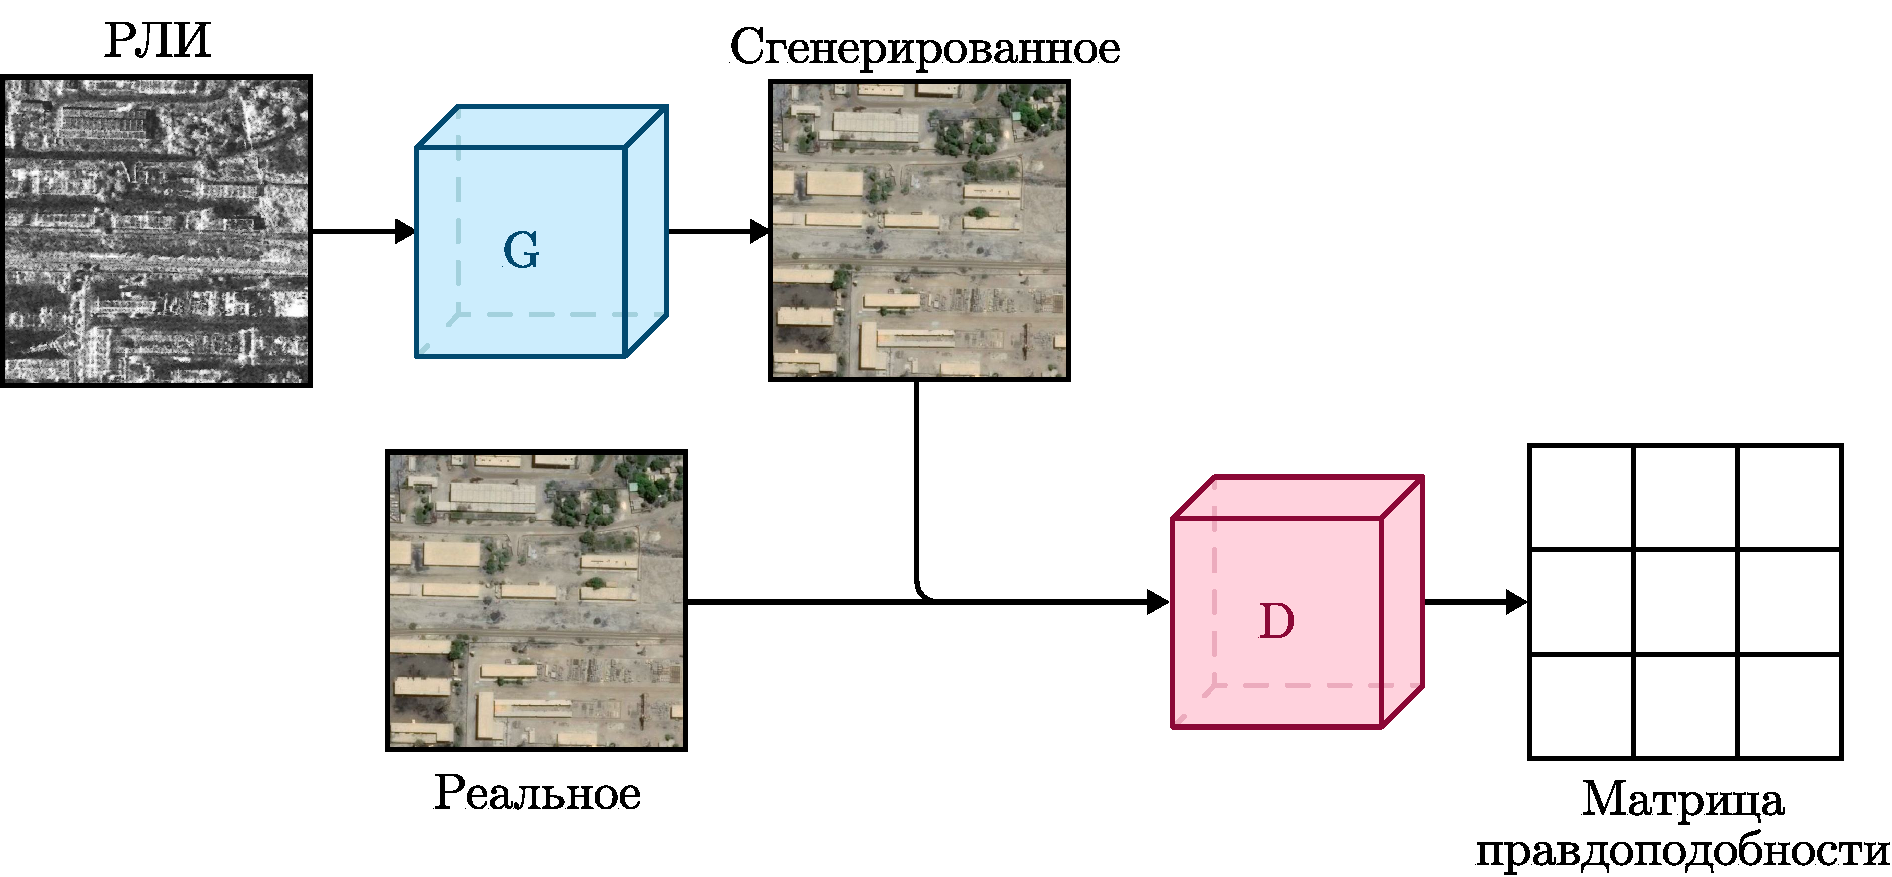
\includegraphics[width=1\linewidth]{images/pix2pix/Pix2Pix.pdf}
    \caption{Архитектура Pix2Pix}
    \label{fig:pix2pix_arch}
\end{figure}

Генератор реализован в виде U-Net \cite{cciccek20163d}(рис.~\ref{fig:unet_arch}) -- свёрточной архитектуры «кодер–декодер» с пропускаемыми связями (skip connections) между симметричными слоями. Пропускаемые связи позволяют напрямую передавать низкоуровневые признаки из кодировщика в декодировщик, что критически важно для сохранения пространственной структуры объектов, которая у РЛИ и оптических снимков частично совпадает (границы полей, городские кварталы, дороги).

Дискриминатор (рис.~\ref{fig:patchGAN}) представляет собой свёрточный классификатор типа PatchGAN: он разбивает изображение на перекрывающиеся участки фиксированного размера (N×N пикселей) и выносит решение о подлинности для каждого из них независимо. Такой подход штрафует высокочастотные артефакты на малых масштабах и требует существенно меньше параметров, чем полносвязный дискриминатор на всё изображение.

\begin{figure}[!ht]
    \centering
    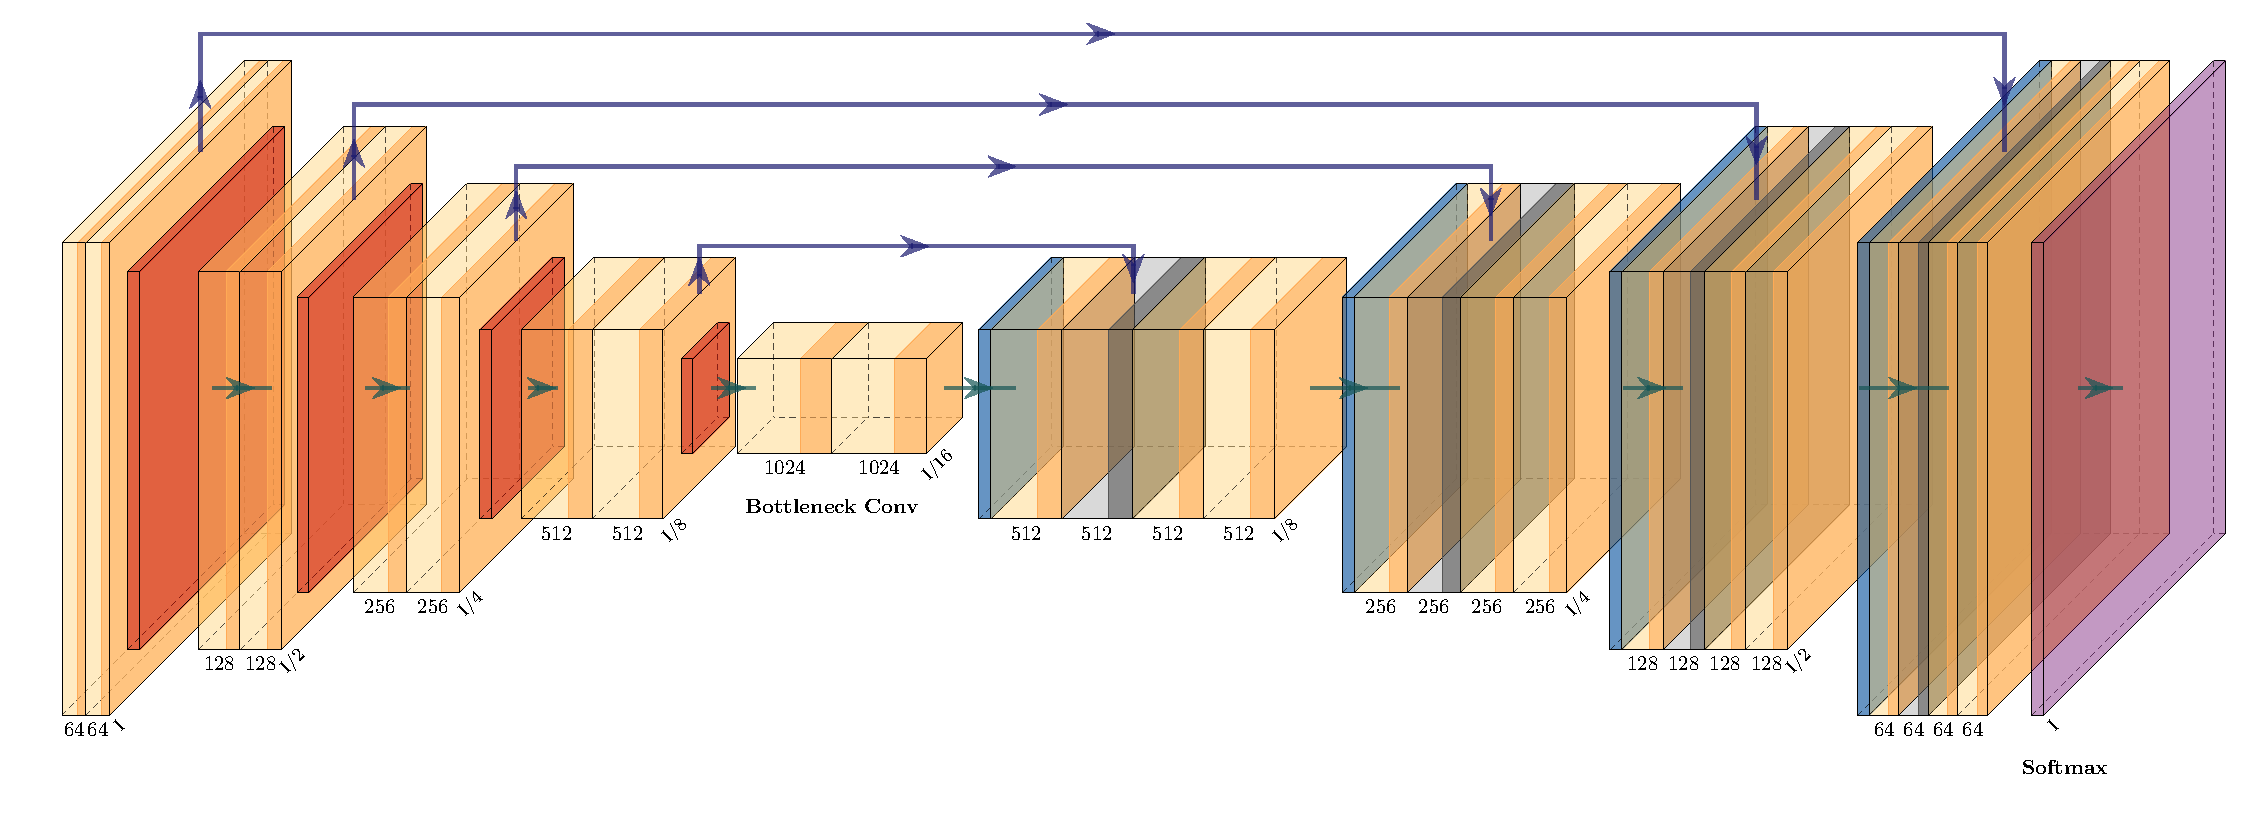
\includegraphics[width=1\linewidth]{images/pix2pix/u-net-architecture.pdf}
    \caption{Архитектура UNet}
    \label{fig:unet_arch}
\end{figure}

\begin{figure}[!ht]
    \centering
    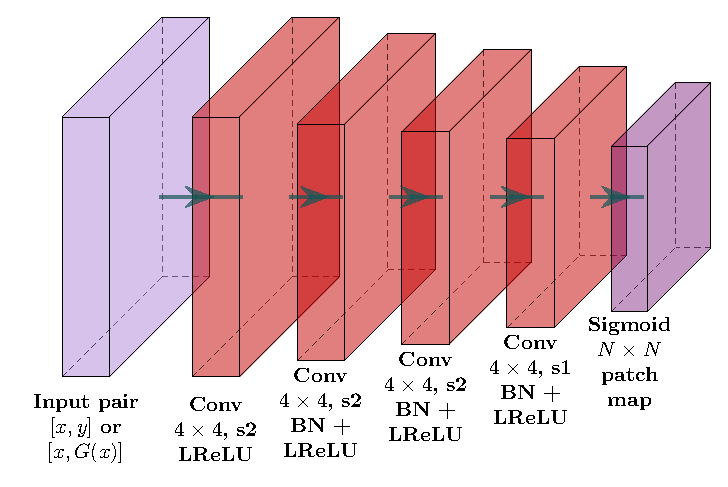
\includegraphics[width=0.5\linewidth]{images/pix2pix/patchGAN.pdf}
    \caption{Архитектура PatchGAN}
    \label{fig:patchGAN}
\end{figure}

Целевая функция состоит из двух слагаемых. Первое – условная состязательная потеря (cGAN loss)~\ref{eq:adv_loss} стимулирует генератор создавать изображения, которые дискриминатор не сможет отличить от реальных. Второе – пиксельная L1-норма~\ref{eq:l1_l2}, которая поощряет точное воспроизведение контуров и текстур. Совместная функция потерь имеет вид:
\begin{equation}
    Loss = \mathcal{L}_{\mathrm{cGAN}}(G, D) + \lambda \, \mathbb{E}_{x, y}[\|y - G(x)\|_1],
\end{equation}

где $\lambda$ – гиперпараметр, регулирующий баланс между фотореалистичностью и попиксельной точностью (обычно $\lambda = 100$). L1-норма выбрана вместо L2, так как она даёт меньше размытых предсказаний и лучше сохраняет контрастные границы.

Обучение происходит итеративно: на каждом шаге сначала обновляются веса дискриминатора, а затем генератора. Необходим тщательный подбор скорости обучения и размера батча, чтобы избежать доминирования одного из игроков.

\subsection{Применение к SAR-изображениям и типовые ограничения}

Пионерские работы по переводу SAR→оптика с помощью Pix2Pix показали принципиальную возможность восстановления пространственного расположения объектов и даже крупных текстур, неразличимых на исходном радарном снимке. Однако при детальном анализе выявляется ряд фундаментальных и технических ограничений, присущих данной архитектуре в контексте SAR.

\begin{enumerate}
    \item \textbf{Замыливание высокочастотных деталей.} Несмотря на наличие skip-connections, результирующие изображения часто страдают от недостатка чёткости. Границы объектов (береговые линии, контуры зданий) выглядят размытыми. Это является прямым следствием минимизации L1-нормы, которая поощряет генератор выдавать «усреднённое» предсказание, сглаживающее острые перепады яркости. В случае SAR-изображений, где многие объекты представлены в виде текстурных паттернов, это приводит к существенной потере информации.
    \item \textbf{Потеря мелких объектов.} Малоразмерные элементы сцены -- автомобили, небольшие строения, отдельно стоящие деревья -- часто либо исчезают вовсе, либо сливаются с фоном. Это особенно критично для датасета QXS-SAROPT с его разнообразием типов подстилающей поверхности, где мелкие объекты могут быть ключевыми для интерпретации сцены.
    \item \textbf{Сложности с обучением.} Модель может испытывать трудности с сходимостью, особенно при работе с высокоразмерными изображениями и ограниченным количеством парных данных. Нерегулярные градиенты и колебания в процессе обучения могут приводить к нестабильным результатам.
    \item \textbf{Ограниченная способность к генерализации.} Модель, обученная на одном типе местности (например, сельской), может плохо справляться с другой (городской), что указывает на недостаточную способность к обобщению и необходимость в более сложных архитектурных решениях.
    \item \textbf{Зависимость от качества парных данных.} Pix2Pix требует строго выровненных пар SAR-оптика для обучения. Наличие шумов, геометрических искажений или временных разрывов в данных может существенно ухудшить качество генерации.
\end{enumerate}

\section{Непарные методы: CycleGAN}
\label{sec:cyclegan}

Дефицит точно зарегистрированных пар SAR--optical, обусловленный различиями в орбитальной геометрии, погодными ограничениями и временными рассогласованиями съёмок, стимулировал развитие непарных (unpaired) методов трансфера. Базовой архитектурой в этом направлении стала CycleGAN~\cite{zhu2017unpaired} (рис.~\ref{fig:cyclegan_arch}), позволяющая обучать отображение между доменами без попарного соответствия пикселей. Несмотря на высокую гибкость, прямое применение CycleGAN к радиолокационным данным выявило ряд фундаментальных ограничений, связанных с физической некорректностью задачи раскраски, когерентным шумом и структурной асимметрией модальностей. В связи с этим современные исследования сосредоточены на стратегиях стабилизации обучения и регуляризации целевой функции.

\begin{figure}[!ht]
    \centering
    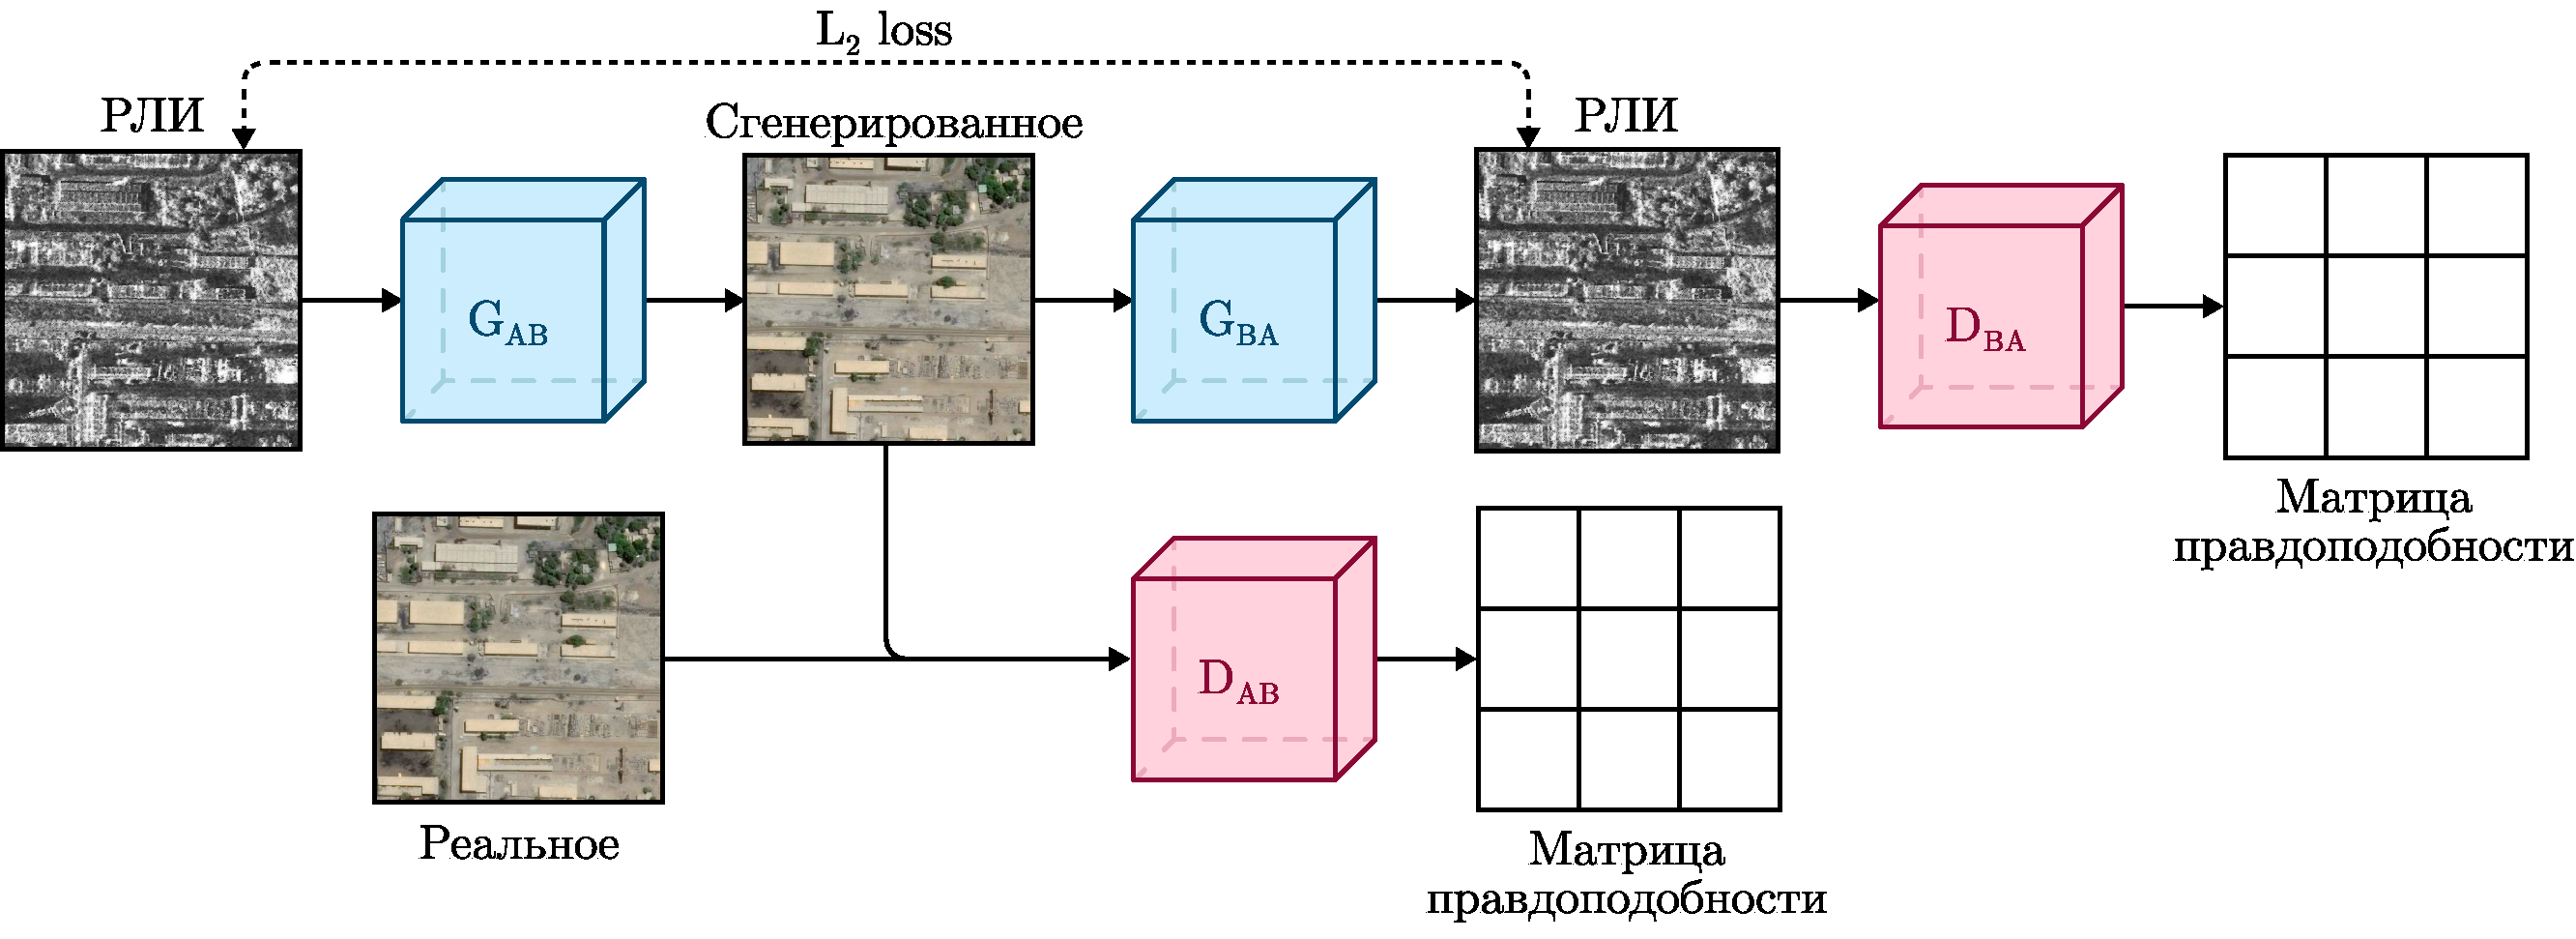
\includegraphics[width=1\linewidth]{images/cyclegan/CycleGAN.pdf}
    \caption{Архитектура CycleGAN}
    \label{fig:cyclegan_arch}
\end{figure}

\subsection{Принцип циклической согласованности}
CycleGAN формулирует задачу как двунаправленный трансфер между доменами $A$ (SAR) и $B$ (Optical) с использованием двух генераторов $G_{AB}:  A\to B$, $G_{BA}: B \to A$ и двух дискриминаторов $D_{AB}$, $D_{BA}$. Обучение опирается на состязательные потери в каждом направлении:
\begin{equation}
    \mathcal{L}_{\text{GAN}}(G_{AB}, D_{AB}, A, B) = \mathbb{E}_{b \sim p_{\text{data}}(b)}[\log D_{AB}(b)] + \mathbb{E}_{a \sim p_{\text{data}}(a)}[\log(1 - D_{AB}(G_{AB}(a)))],
\end{equation}
и аналогично для пары $(G_{BA}, D_{BA})$. Ключевым компонентом, предотвращающим произвольное отображение и коллапс моды, является потеря циклической согласованности (cycle-consistency loss):
\begin{equation}
    \mathcal{L}_{\text{cyc}}(G_{AB}, G_{BA}) = \mathbb{E}_{a \sim p_{\text{data}}(a)}[\|G_{BA}(G_{AB}(a))) - a\|_1] + \mathbb{E}_{b \sim p_{\text{data}}(b)}[\|G_{AB}(G_{BA}(b))) - b\|_1].
\end{equation}
Полная целевая функция имеет вид $\mathcal{L} = \mathcal{L}_{\text{GAN}}(G_{AB}, D_{AB}, A, B) + \mathcal{L}_{\text{GAN}}(G_{BA}, D_{BA}, B, A) + \lambda \mathcal{L}_{\text{cyc}}(G_{AB}, G_{BA})$, где $\lambda$ балансирует вклад цикла~\cite{zhu2017unpaired}. Циклическое ограничение гарантирует, что трансформация сохраняет семантическое содержание исходного изображения, обеспечивая обратимость отображения на уровне распределений. Это позволяет обучать модель на больших массивах независимых РЛИ и оптических снимков, обходя необходимость точной пространственной регистрации и существенно расширяя доступную обучающую выборку.

\subsection{Проблемы цвета, галлюцинаций и структурного коллапса}
Несмотря на теоретическую устойчивость, применение CycleGAN к задаче SAR-to-Optical сопровождается рядом систематических артефактов.
Во-первых, отображение одноканальной радиолокационной интенсивности в трёхканальное цветовое пространство является существенно некорректным (ill-posed), то есть задача не имеет единственного, устойчивого и физически обоснованного решения, что приводит к цветовому дрейфу и хроматическим искажениям, особенно при смене сезонов, типов подстилающей поверхности или условий освещения.
Во-вторых, когерентный шум (speckle) и геометрические искажения SAR (layover, shadowing) нарушают структурное соответствие, вызывая размытие контуров и слияние объектов в плотной городской застройке. 
В-третьих, при дисбалансе распределений доменов или недостаточной регуляризации наблюдается структурный коллапс и галлюцинации: модель может генерировать дороги вместо рек, искажать границы сельскохозяйственных полей или добавлять несуществующие здания. Эти ошибки критичны для прикладных задач дистанционного зондирования, поскольку стандартные метрики (PSNR, SSIM) не фиксируют семантические несоответствия, а визуальная правдоподобность маскирует топологические искажения.
Дополнительно, непарное обучение чувствительно к локальным рассогласованиям и сезонным сдвигам, что усиливает геометрическую нестабильность генерации и провоцирует накопление ошибок в цикле.

Совокупное применение указанных стратегий трансформирует CycleGAN из базовой схемы стилевого переноса в устойчивый каркас для кросс-модального трансфера, способный работать в условиях дефицита парных данных при сохранении структурной и семантической целостности сцены.
Тем не менее, компромисс между гибкостью непарного обучения и точностью пиксельного соответствия остаётся открытой проблемой, мотивирующей развитие staged pretraining, частотных ограничений и РЛИ-осознанных регуляризации.

\section{Архитектурные инновации в GAN для SAR-изображений}
\label{sec:arch_innovations_gan}

Эволюция генеративно-состязательных сетей для задачи SAR-to-Optical сместилась от адаптации универсальных бэкбонов (U-Net, ResNet) к разработке целевых архитектур, учитывающих физику радиолокационного сигнала, многомасштабную природу сцен и высокую степень некорректности кросс-модального отображения.
Ключевым направлением стало преодоление информационных потерь на этапе feature reasoning, подавление когерентного шума без разрушения границ и интеграция внешних геопространственных признаков.
Показательным примером такого перехода является CFRWD-GAN~\cite{wei2023cfrwd}, в которой предложены рассуждение на основе перекрестного слияния и частотно-ориентированная обработка, дополненные в современных работах вспомогательными условиями и физическими ограничениями.

\subsection{Многостадийные и кросс-модальные структуры (CFR, HRNet-подобные схемы)}
Базовые генераторы Pix2Pix и CycleGAN используют U-Net с skip-connections или каскад остаточных блоков (CN-ResBlocks).
Несмотря на простоту, эти схемы страдают от систематических потерь информации: в U-Net конкатенация разноуровневых признаков из энкодера и декодера не обеспечивает содержательного согласования РЛИ и оптических представлений, а CN-ResBlocks выполняют рассуждения (reasoning) только на фиксированном масштабе, что препятствует восстановлению многомасштабной структуры сцены.

Для решения этой проблемы в CFRWD-GAN предложена структура \textit{Cross-Fusion Reasoning (CFR)} (рис.\ref{fig:cfrwd_arch}), вдохновлённая архитектурой HRNet.
CFR сохраняет высокочастотные детальные признаки и низкочастотные семантические представления на протяжении всего процесса reasoning за счёт параллельных многомасштабных ветвей и поэтапного кросс-фьюжна.
Процесс разделён на три стадии: на каждой стадии добавляется новая масштабная ветвь, а выходы предыдущей стадии объединяются через операции повышения/понижения разрешения и конкатенации с последующей свёрткой:

\begin{figure}[!ht]
    \centering
    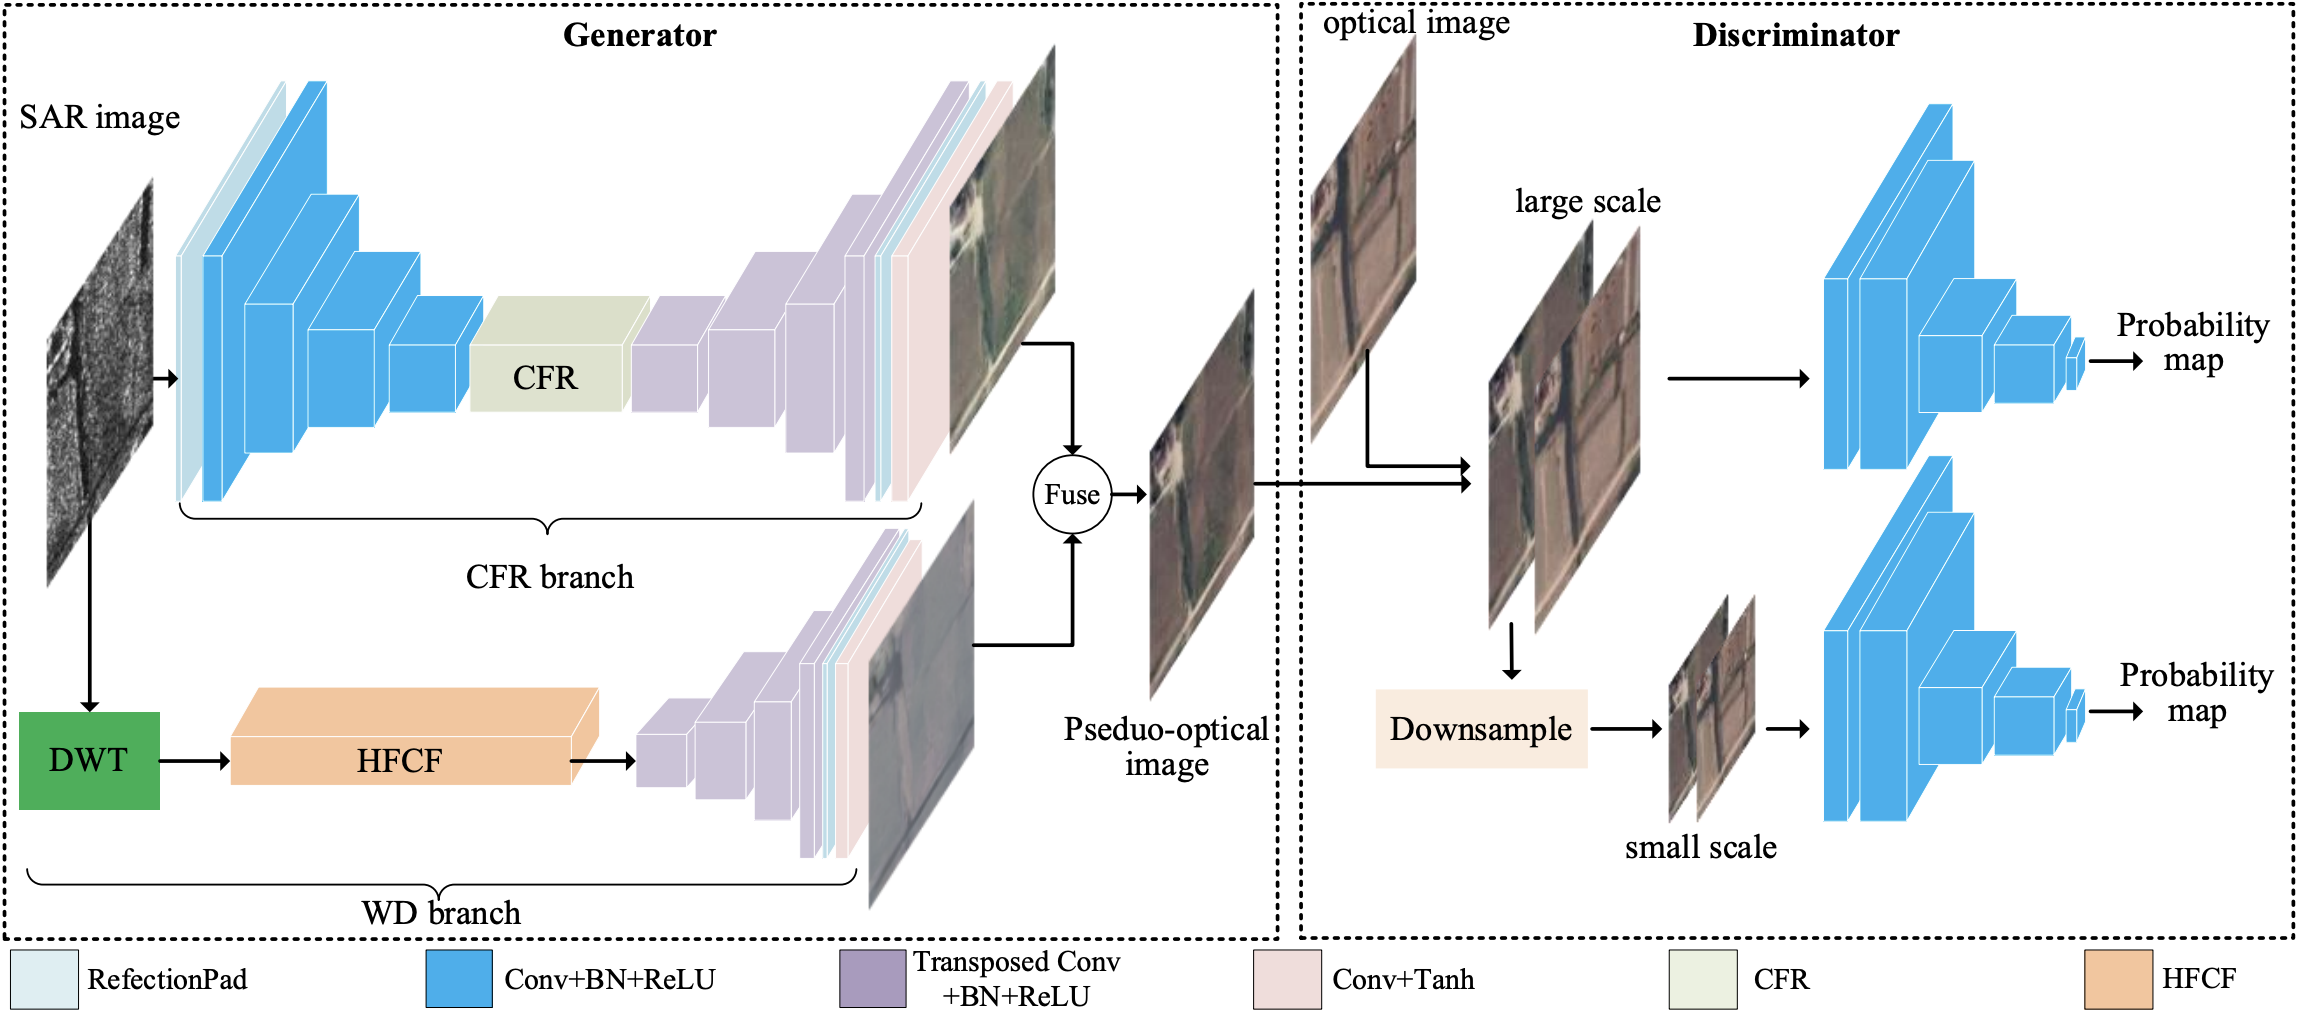
\includegraphics[width=1\linewidth]{images/cfrwd/cfrwd_arch.png}
    \caption{Архитектура CFRWD}
    \label{fig:cfrwd_arch}
\end{figure}

\begin{equation}
    b_1 = \text{Conv}(\text{cat}(p_1, \uparrow p_2)), \quad
    b_2 = \text{Conv}(\text{cat}(\downarrow p_1, p_2)), \quad
    b_3 = \text{Conv}(\text{cat}(\downarrow\downarrow p_1, \downarrow p_2)),
\end{equation}
где $\uparrow$, $\downarrow$ обозначают upsample и downsample, а $p_i$, $b_i$ -- признаки разных масштабов и стадий. Аналогичные операции выполняются на второй и третьей стадиях, после чего все масштабные представления выравниваются по размеру и интегрируются через $1\times1$ свёртку~\cite{wei2023cfrwd}. Визуальное представление можно наблюдать на рис.~\ref{fig:cfr_arch}.

\begin{figure}[H]
    \centering
    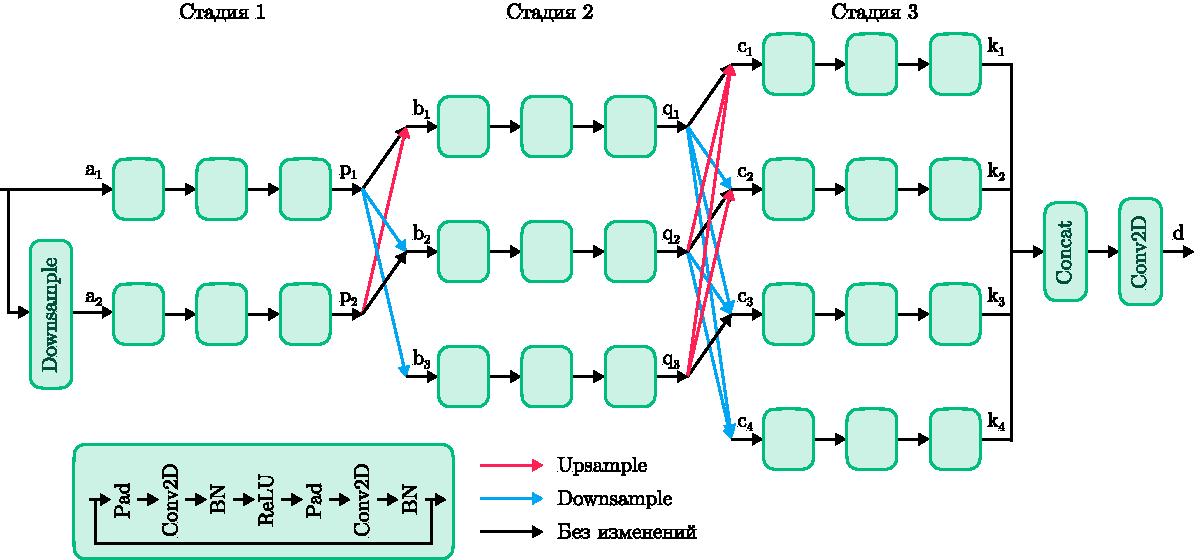
\includegraphics[width=1\linewidth]{images/cfrwd/CFR.pdf}
    \caption{Архитектура CFR}
    \label{fig:cfr_arch}
\end{figure}

Такая организация позволяет:
\begin{itemize}
    \item избегать информационного коллапса при переходе между масштабами;
    \item выполнять поэтапный перевод SAR-признаков в оптические с сохранением топологии линейных объектов (дорог, рек) и контуров застройки;
    \item стабилизировать градиенты за счёт горизонтального углубления и вертикального расширения сети.
\end{itemize}
Визуализация карт признаков подтверждает, что CFR сохраняет существенно больше структурной информации по сравнению с U-Net и CN-ResBlocks, что напрямую отражается на улучшении метрик SSIM и LPIPS~\cite{wei2023cfrwd}.

\subsubsection{Частотные и вейвлет-ориентированные подходы}
Когерентный шум (speckle) в РЛИ концентрируется в высокочастотных компонентах, одновременно маскируя границы и мелкие детали. Прямая пространственная фильтрация или обучение в пиксельном пространстве часто приводит к чрезмерному сглаживанию или переносу шумовых артефактов в оптический домен. Частотно-ориентированные архитектуры решают эту проблему за счёт явного разделения спектральных полос и независимой обработки высокочастотных подполос~\cite{wei2023cfrwd}.

В CFRWD-GAN реализована \textit{Wavelet Decomposition (WD) branch} (рис.\ref{fig:wd}), выполняющая двумерное вейвлет-разложение (Haar, 2 уровня) входного SAR-изображения на семь компонент: низкочастотную $LL_2$ и высокочастотные $\{LH_2, HL_2, HH_2\}$, $\{LH_1, HL_1, HH_1\}$.
Высокочастотные подполосы содержат контуры и текстуры, но также несут основную долю speckle-шума.
Для их обработки предложен модуль \textit{High-Frequency Coding and Filtering (HFCF)}, построенный на остаточных блоках ResNet-типа, который подавляет шум в вейвлет-домене и восстанавливает оптически согласованные высокочастотные признаки.
Декодирование отфильтрованных компонент формирует детальную карту границ, которая затем объединяется с выходом CFR-ветви через обучаемый коэффициент слияния~\cite{wei2023cfrwd}.

\begin{figure}[!ht]
    \centering
    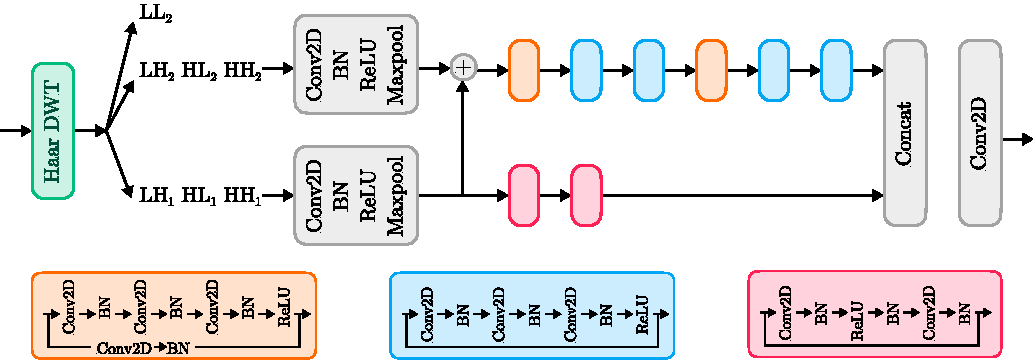
\includegraphics[width=1\linewidth]{images/cfrwd/WD.pdf}
    \caption{Архитектура WD}
    \label{fig:wd}
\end{figure}

Преимущества частотного подхода:
\begin{itemize}
    \item явное разделение структуры (низкие частоты) и деталей/шума (высокие частоты);
    \item подавление speckle без размытия геометрических границ;
    \item улучшение восстановления тонких линейных объектов и текстур растительности/застройки.
\end{itemize}
Вейвлет-ориентированные схемы стали одним из ключевых трендов в SAR-to-Optical GAN. Помимо CFRWD-GAN, исследуются DCT-остаточные блоки для частотной регуляризации~\cite{guo2022sar2color}, wavelet-guided discriminator~\cite{george2022wavelet}, spatial-frequency complementary learning в диффузионных моделях~\cite{qin2024conditional} и frequency-domain ограничения для стабилизации цикла в непарных схемах~\cite{wang2025generative}. Комбинация многомасштабного reasoning и частотной обработки демонстрирует наилучший компромисс между структурной целостностью и перцептивным качеством.

\subsubsection{Вспомогательные условия и физические априорные данные}
Отображение SAR$\to$Optical является существенно некорректным: одноканальная радиолокационная интенсивность не содержит однозначной информации о цвете, сезонности, рельефе или классе покрытия. Для снижения неопределённости современные архитектуры интегрируют вспомогательные условия и физические priors, выступающие как геометрические, семантические или радиометрические якоря~\cite{wang2025generative}.

Основные типы априорных данных и стратегии их интеграции:
\begin{itemize}
    \item \textbf{Картографические и семантические priors:} OpenStreetMap (OSM), LULC-карты и маски классов сцен используются как дополнительные каналы входа или условия для auxiliary branches, стабилизируя геометрию дорог, зданий и гидрографии~\cite{cabrera2021sar, fu2024advanced, guo2024scene}.
    \item \textbf{Рельеф и высота:} DEM и LiDAR позволяют корректировать геометрические искажения SAR (layover, foreshortening, shadowing) и компенсировать рельефно-обусловленные цветовые сдвиги. Интеграция осуществляется через encoder-decoder conditioning или physics-informed потери~\cite{zhu2024fusing, bralet2024dem, zhang2024interpretable}.
    \item \textbf{Мультитемпоральная информация:} соседние по времени SAR/optical снимки, маски облачности и seasonal embeddings используются для согласования временных сдвигов, стабилизации цвета и восстановления закрытых облаками регионов. Реализуется через temporal co-attention, cross-date dependency modules и staged pretraining~\cite{kwak2024assessing, liu2022modality, wang2025generative}.
    \item \textbf{Параметры съёмки:} угол падения (incidence angle), поляризация (VV/VH/HH) и частотный диапазон включаются как метаданные или positional encoding, улучшая радиометрическую согласованность и обобщающую способность модели~\cite{wang2025generative}.
\end{itemize}

Интеграция priors снижает степень ill-posedness, уменьшает галлюцинации и улучшает спектральную устойчивость, особенно в сложных ландшафтах и при сезонных сдвигах. Однако это увеличивает зависимость от доступности внешних данных, усложняет pipeline и требует тщательной пространственной регистрации. Перспективным направлением является \textit{task-aware conditioning}, где вспомогательные признаки оптимизируются совместно с downstream-задачами (сегментация, детекция, регистрация), обеспечивая семантически согласованный трансфер без избыточной зависимости от ручных priors~\cite{wang2025generative, zhang2025seg}.

Совокупное применение CFR-подобных многомасштабных структур, частотной обработки и вспомогательных условий формирует современный стандарт архитектурного дизайна GAN для SAR-to-Optical. Эти инновации напрямую адресуют ключевые ограничения базовых схем: информационные потери при reasoning, speckle-индуцированное размытие границ и цветовую/семантическую неоднозначность кросс-модального отображения.

\section{Трансформеры и гибридные CNN--Transformer архитектуры}
\label{sec:transformers_sar2opt}

Свёрточные нейронные сети долгое время доминировали в задачах кросс-модального перевода, однако их архитектурные ограничения стали заметным барьером при переходе от стилистического переноса к физически обоснованному трансферу SAR--optical. Внедрение механизмов самовнимания и трансформерных бэкбонов позволило преодолеть ряд фундаментальных проблем, связанных с моделированием глобального контекста, сохранением топологии и подавлением семантических галлюцинаций.

\subsubsection{Ограничения свёрточных сетей в кросс-модальном переводе}
Базовые генераторы на основе CNN оперируют локальным рецептивным полем, что ограничивает их способность моделировать долгосрочные зависимости и глобальную структуру сцены. В задаче SAR-to-Optical это проявляется в нескольких систематических артефактах:
\begin{itemize}
    \item \textbf{Размытие линейных и протяжённых объектов:} дороги, реки, границы полей и инфраструктурные сети теряют связность, поскольку свёрточные ядра не обеспечивают согласования удалённых фрагментов~\cite{wang2025generative, kong2022multi}.
    \item \textbf{Семантический дрейф и галлюцинации:} из-за отсутствия глобального контекста модель может генерировать правдоподобные локальные текстуры, но нарушать топологию (например, отображать русла рек как дорожную сеть или фрагментировать застройку)~\cite{wang2025generative, luo2024contextual}.
    \item \textbf{Чувствительность к рассогласованию и speckle-шуму:} локальные операции усиливают влияние когерентного шума на feature reasoning, что приводит к накоплению ошибок при переходе между масштабами и нестабильности adversarial-обучения~\cite{wei2023cfrwd, wang2025generative}.
\end{itemize}
Эти ограничения мотивировали переход к архитектурам, способным явно моделировать non-local зависимости и выравнивать кросс-модальные представления на уровне глобальной сцены.

\subsubsection{Интеграция Vision Transformer и Swin-Transformer в генераторы}
Прямое применение Vision Transformer (ViT) в SAR-to-Optical ограничено высокой вычислительной сложностью квадратичного внимания и требовательностью к объёму обучающих данных. Практическим компромиссом стали иерархические и оконные варианты, в первую очередь Swin-Transformer, а также гибридные CNN--ViT схемы~\cite{wang2025generative}.

\begin{itemize}
    \item \textbf{Swin-Transformer в генераторах CGAN.} Kong et al.~\cite{kong2022multi} заменили стандартные остаточные блоки на Swin-блоки с shifted window attention. Иерархическое представление и локальное окно внимания позволяют восстанавливать границы и кросс-масштабный контекст без квадратичного роста сложности, что особенно эффективно для сохранения контуров застройки и линейных объектов.
    \item \textbf{Гибридные CNN--ViT архитектуры.} Wang et al.~\cite{wang2022hybrid} и Zhao et al.~\cite{zhao2025hvt} интегрировали CNN-энкодеры для извлечения локальных текстур с ViT-модулями для глобального reasoning. Связь между ветвями осуществляется через multiscale feature propagation paths и convolutional attention modules, что обеспечивает совместное моделирование мелкомасштабных деталей и крупномасштабной семантики. Такие схемы демонстрируют улучшение метрик LPIPS и FID при сохранении приемлемого времени инференса.
    \item \textbf{Трансформеры в диффузионных и последовательных моделях.} В латентных диффузионных каркасах трансформерные блоки используются для условного моделирования временных рядов и пространственно-временных зависимостей. Wei et al.~\cite{wei2025sequential} применили alternating spatiotemporal Transformers с timestep-эмбеддингами для последовательного SAR-to-optical перевода, улучшая стабильность цвета и геометрии в мультитемпоральных сценариях.
\end{itemize}

\subsubsection{Контекстные и кросс-attention модули для SAR--Optical}
Помимо замены бэкбонов, механизмы внимания активно внедряются как целевые модули согласования модальностей и контекста:
\begin{itemize}
    \item \textbf{Contextual Inference Transformer.} Luo et al.~\cite{luo2024contextual} предложили модуль, объединяющий статический контекст (глобальная компоновка сцены) и динамический контекст (локальные текстурные паттерны) для захвата non-local зависимостей. Механизм sharpening edges на основе внимания подавляет артефакты в высокочастотных зонах и улучшает восстановление границ без явного частотного разложения.
    \item \textbf{Кросс-attention между модальностями.} Cross-attention слои используются для выравнивания SAR-структурных priors и оптических текстурно-цветовых распределений. Запрос (query) формируется из SAR-признаков, а ключи/значения (key/value) -- из оптических или вспомогательных представлений, что снижает галлюцинации и якорит семантику целевого домена~\cite{wang2025generative, zhao2025hvt}.
    \item \textbf{Временное и междоменное внимание.} В мультитемпоральных постановках temporal co-attention и cross-date dependency modules согласовывают сезонные сдвиги, геометрию съёмки и изменения покрытия, направляя генерацию в сложных сценариях с облачностью или фенологическими переходами~\cite{kwak2024assessing, liu2022modality}.
\end{itemize}

\subsubsection{Преимущества, вычислительные компромиссы и открытые вопросы}
Интеграция трансформеров в SAR-to-Optical pipelines демонстрирует ряд устойчивых преимуществ:
\begin{itemize}
    \item лучшая сохранность топологии и связности линейных объектов;
    \item повышенная устойчивость к локальным рассогласованиям и сезонным сдвигам;
    \item улучшение семантической согласованности и снижение частоты структурных галлюцинаций;
    \item эффективное моделирование кросс-модального контекста без жёстких пиксельных ограничений.
\end{itemize}

Однако эти преимущества сопровождаются существенными компромиссами:
\begin{itemize}
    \item \textbf{Вычислительная и память-ёмкость:} даже оконные и гибридные схемы требуют значительных ресурсов при разрешениях $256\times256$ и выше, что ограничивает применение на бортовых или edge-платформах~\cite{wang2025generative}.
    \item \textbf{Чувствительность к данным и регуляризации:} трансформеры склонны к переобучению при малых выборках и требуют тщательной аугментации, positional encoding, адаптированного к геопространственным координатам, и стабилизации adversarial-градиентов~\cite{zhao2025hvt, wang2025generative}.
    \item \textbf{Интеграция с физическими priors:} стандартные attention-механизмы не учитывают радиолокационную физику (incidence angle, поляризацию, рельефные искажения), что требует разработки geometry-aware и frequency-conditioned attention модулей.
\end{itemize}

\textbf{Открытые исследовательские вопросы} включают: разработку облегчённых attention-вариантов (linear, sparse, state-space) для дистанционного зондирования; создание task-aware трансформеров, совместно оптимизирующих перевод и downstream-задачи (сегментация, детекция); стандартизацию бенчмарков для оценки семантической целостности трансформерных генераторов; и интеграцию кросс-attention с диффузионными мостами для стабильного непарного трансфера~\cite{wang2025generative}. Указанные направления определяют вектор развития архитектур следующего поколения, где глобальное контекстное моделирование сочетается с частотной, физической и семантической регуляризацией.

\section{Сравнительная оценка моделей трансляции SAR--Optical на датасетах SEN-12 и QXS-SAROPT}

\begin{table}[!ht]
\centering
\caption{Сравнительная оценка моделей трансляции SAR--Optical на датасетах SEN-12 и QXS-SAROPT}
\label{tab:sar_optical_comparison}
\begin{tabular}{|l|l|l|l|l|l|l|l|l|}
\hline \multirow[t]{2}{*}{Model} & \multicolumn{4}{|l|}{SEN-12} & \multicolumn{4}{|l|}{QXS-SAROPT} \\
\hline & PSNR (dB) ↑ & SSIM ↑ & LPIPS ↓ & FID ↓ & PSNR (dB) ↑ & SSIM ↑ & LPIPS ↓ & FID  \\
\hline Pix2Pix & 12.79 & 0.1793 & 0.4834 & 113.87 & 13.28 & 0.2980 & 0.5316 & 135.72 \\
\hline INRECGAN & 15.74 & 0.2934 & 0.4613 & 73.96 & 15.86 & 0.3892 & 0.4672 & 92.06 \\
\hline CycleGAN & 11.54 & 0.1717 & 0.4974 & 89.38 & 13.67 & 0.2747 & 0.6024 & 185.75 \\
\hline ScE-GAN & 11.04 & 0.1721 & 0.5173 & 78.94 & 12.49 & 0.3161 & 0.6572 & 174.44 \\
\hline DTGAN & 13.52 & 0.1939 & 0.5266 & 82.41 & 14.67 & 0.3179 & 0.5131 & 69.89 \\
\hline DDA-GAN & 11.69 & 0.1743 & 0.4990 & 87.14 & 13.85 & 0.2784 & 0.5872 & 208.64 \\
\hline S20CDM & 12.76 & 0.3008 & 0.4554 & 70.84 & 12.46 & 0.3233 & 0.5179 & 62.39 \\
\hline $E^3$ Diff & 18.84 & 0.4213 & 0.3664 & 65.23 & 18.62 & 0.4475 & 0.3411 & 52.87 \\
\hline
\end{tabular}
\end{table}

\begin{figure}[!ht]
    \centering
    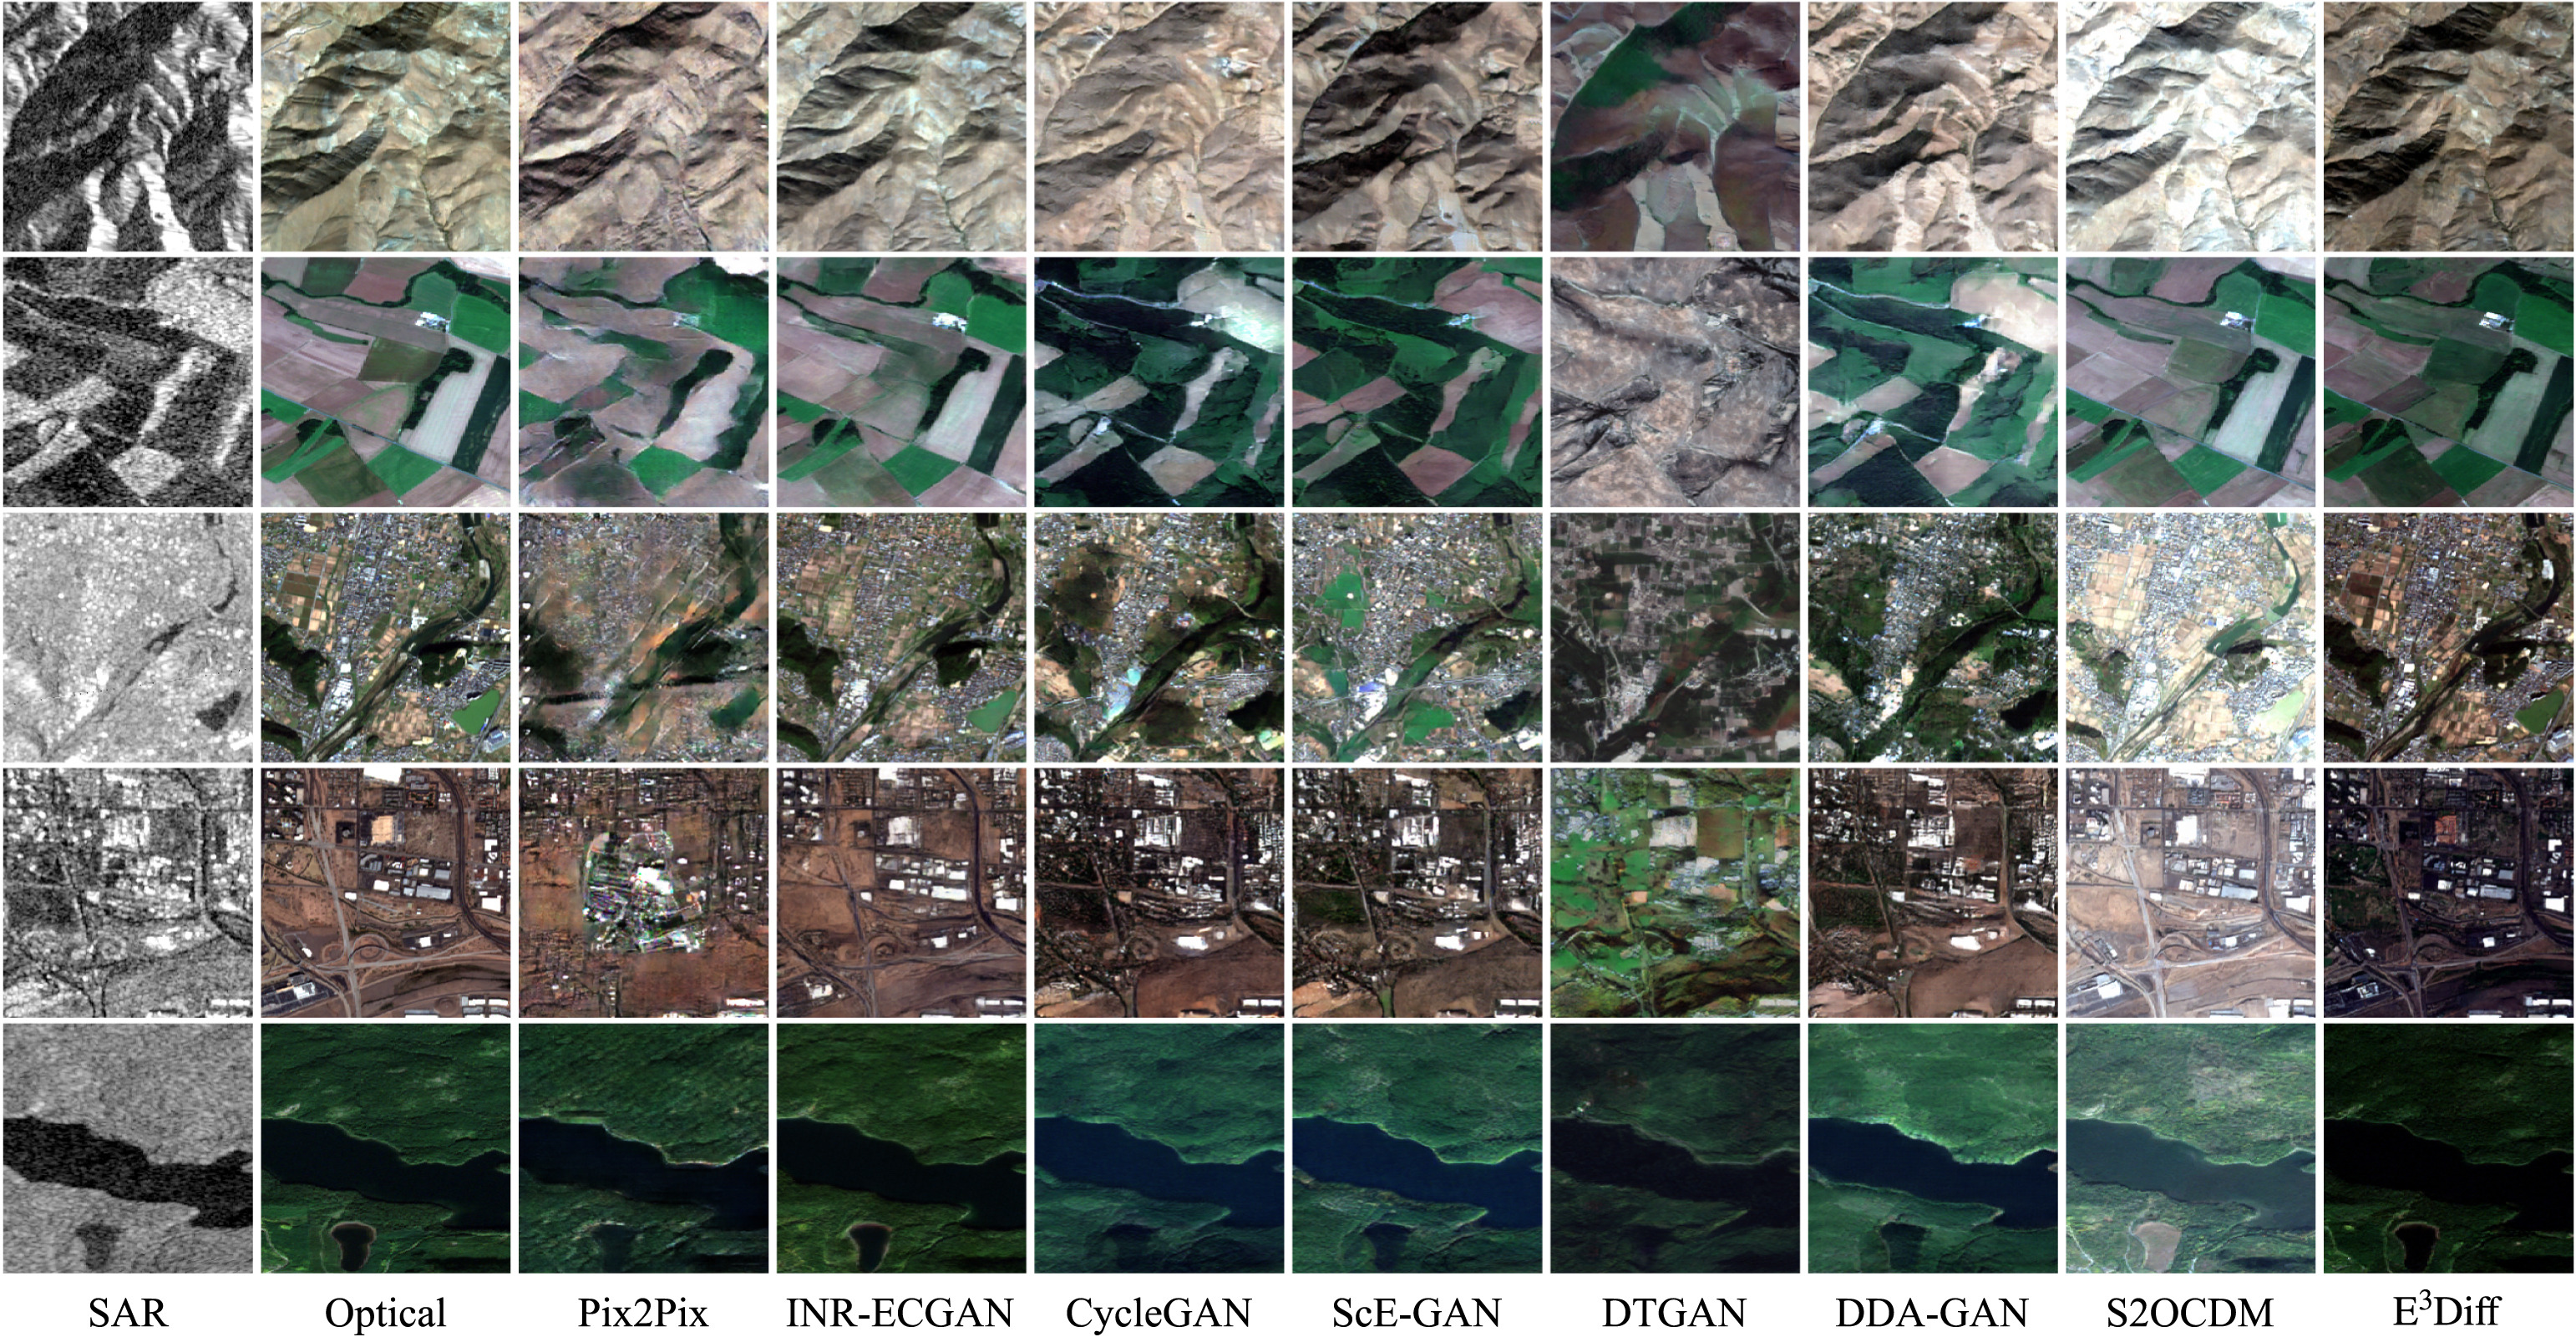
\includegraphics[width=1\linewidth]{images/all_models_comparison.jpg}
    \caption{Сравнение моделей трансляции SAR--Optical}
    \label{fig:all_models_comparison}
\end{figure}

\newpage